\chapter{Architektury přístupových systémů}

Přístupové systémy jsou elektronické systémy řídící přístup uživatelů do omezených prostor v závislosti na jejich prokázané identitě.

\begin{figure}[!h]
    \centering
    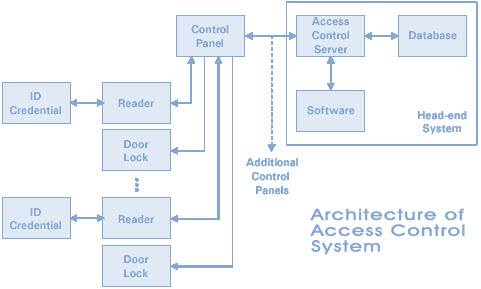
\includegraphics[width=130mm]{Architetcture-of-Access-Control-System}
    \caption{Příklad architektury přístupového systému \cite{accessControlSystem_eiprocus}}
    \label{fig:Access control system architecture}
\end{figure}

Obrázek \ref{fig:Access control system architecture} zobrazuje typickou architekturu přístupového systému, kde ID Credential představuje prvek umožňující identifikovat uživatele, např. RFID tag, otisk prstu nebo QR kód. 
Zařízení typu Reader slouží ke čtení dat z ID Credential a v digitální podobě je odesílá k zařízení typu Control Panel.
Zařízení typu Door Lock řídí fyzický přístup uživatelů do omezených prostor. 
Zařízení typu Control Panel tvoří rozhranní mezi Access Control Server a páry zařízení typů Reader a Door Lock. 
Zařízení typu Control Panel jsou obvykle připojena 
k zařízení typu Access Control Server přes TCP/IP síť a páry zařízení typů Reader a Door Lock jsou obvykle připojeny k zařízení typu Control panel přes RS485 síť. Databáze obsahuje všechna uživatelské ID.
Na Access Control Serveru je spuštěn Software (SW) spravující databázi a komunikující se všemi zařízeními typu Contril Panel.
Zařízení typu Reader čte uživatelská ID z předložených ID Credential a přeposílá je k zařízení typu Control Panel, které je dále přeposílá na Access Control Server. 
Access Control Software vyhledá obdržená uživatelská ID v databázi a pokud je nalezeno, pošle příkaz odpovídajícímu zařízení typu Control Panel k přepnutí odpovídajícímu zařízení typu Door Lock, čímž je uživateli udělen přístup do omezené oblasti \cite{accessControlSystem_eiprocus}.
